\section{Components}\label{ch:CD}

All the calculation in the report until this point were done assuming all components were ideal. Since it was concluded the 2Nx Multilevel BC is the topology that will be build in hardware, we will need to calculate the expected drops as well, to see if the real results are close to the simulations we have ran. 
The same structure will be followed as the previous section, where a 3x non-inverting BC will be analysed and the calculations will be mirrored to achieve the 2Nx combination.

The components considered significant are diodes and switches.Other research papers (REFERENCE SANJEE AND ROSAS CARO) assume the drops across the two are equal. Our goal is two separate the two to improve the accuracy of the model. Since the voltage drop is constant and can be measured (usually also denoted in specification sheets), the rest of the losses can be accounted to the switch.

\subsection{3x Non-inverting}

\begin{figure}[H]%
    \centering
    \subfloat[Switch S\textsubscript{1} ON, Switch S\textsubscript{2} ON\label{CTLBC_ONON}]
    {{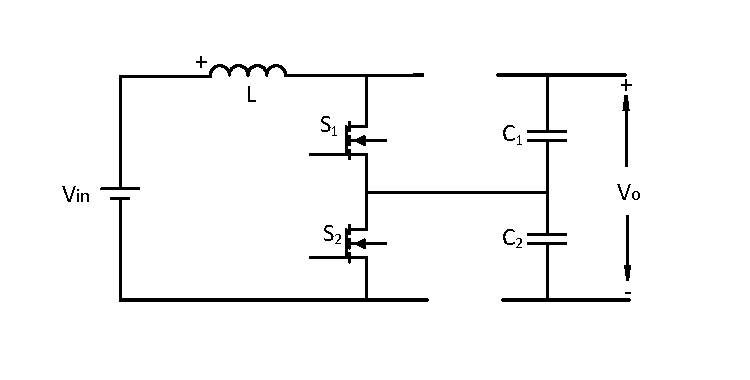
\includegraphics[width=0.45\textwidth]{figures/dConventionalThreeLevelBC/Three_levelONON.pdf} }}%
    \qquad
    \subfloat[Switch S\textsubscript{1} ON, Switch S\textsubscript{2} OFF\label{CTLBC_ONOFF}]{{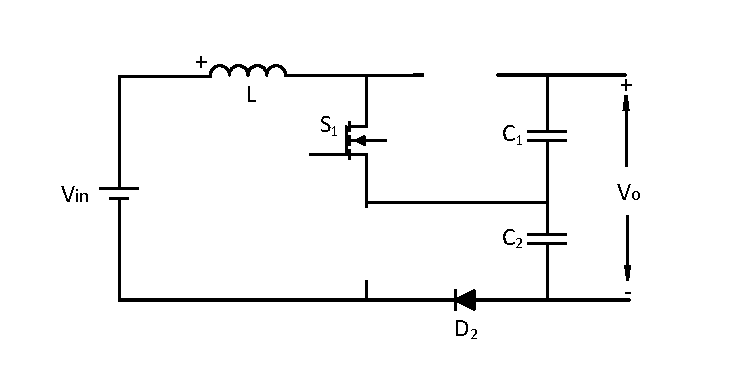
\includegraphics[width=0.45\textwidth]{figures/dConventionalThreeLevelBC/Three_levelONOFF.pdf} }}%  
   \qquad
        \subfloat[Switch S\textsubscript{1} OFF, Switch S\textsubscript{2} ON\label{CTLBC_OFFON}]
    {{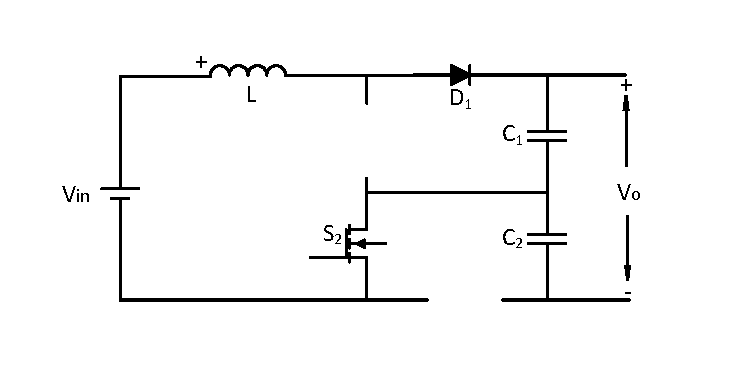
\includegraphics[width=0.45\textwidth]{figures/dConventionalThreeLevelBC/Three_levelOFFON.pdf} }}%
    \qquad
    \subfloat[Switch S\textsubscript{1} OFF, Switch S\textsubscript{2} OFF\label{CTLBC_OFFOFF}]{{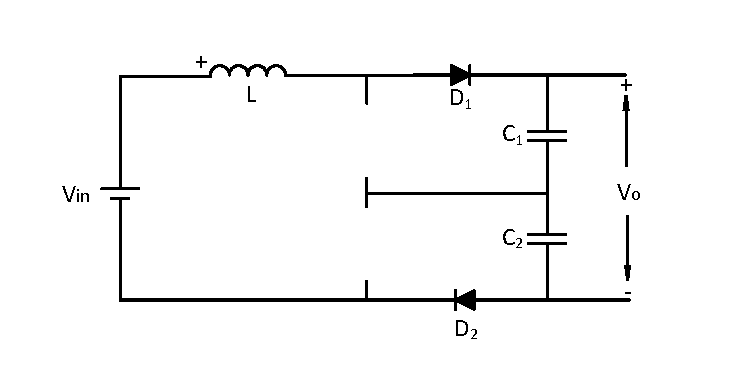
\includegraphics[width=0.45\textwidth]{figures/dConventionalThreeLevelBC/Three_levelOFFOFF.pdf} }}%  
    \caption{Switching states of the SIBC}%
     \label{fig:CTLBC_States}% 
     
\end{figure}